\documentclass[10pt,  english, makeidx, a4paper, titlepage, oneside]{book}
\usepackage{babel}
\usepackage{fancyhdr}
\usepackage{makeidx}
\usepackage{titlesec}
\usepackage{listings} 


\newenvironment{listato}{\footnotesize}
                        {\normalsize }


%\pagestyle{empty}

\textwidth 15.5cm
\textheight 23cm
\topmargin -1cm
\oddsidemargin -0.5cm
\linespread{1.1}

\pagestyle{fancy}
\lhead{}
\chead{Integrated Systems Architecture}
\lfoot{}
\cfoot{}
\rfoot{}
\rhead{\thepage}

\usepackage{graphicx}
\usepackage{amsmath}
\usepackage{amsfonts}
\usepackage{amsthm}
\usepackage{amssymb}
%\oddsidemargin -1.1cm

\titleformat{\chapter}[display]
{\normalfont\Large\filcenter\sffamily}
{\titlerule[0.5pt]%
\vspace{1pt}
\titlerule
\vspace{1pc}
\LARGE\MakeUppercase{\chaptertitlename} \thechapter
}
{1pc}
{\titlerule
\vspace{1pc}
\Huge}

\newcommand{\SubSubSection}[1]{\subsubsection{\bf Exercise   ~#1}}

\newcommand{\homework}[1]{\subsubsection{\bf Homework   ~#1}}

\newcommand{\Solution}{\subsubsection{\bf Solution}}




\makeindex
\begin{document}
\frontmatter
\begin{titlepage}
\vspace{2cm}
\centerline{

\includegraphics[width=2cm]{./logopoli}}  
\centerline{\LARGE Politecnico di Torino}
\bigskip
\centerline{\Large III Facolt\`a di Ingegneria}
\vspace{4cm}
\centerline{\Huge\sf Report Lab3}
\bigskip
\centerline{\Huge\bfseries\sf Integrated Systems Architecture}
\vspace{2cm}
\centerline{\LARGE Master degree in Electrical Engineering}
\vspace{4.4cm}
%%%%%%%%%%%%%%%%%%%%%%%%%%%%%%%%%%%%%%%%%%%%%%%%%%%%%%%
% GROUP
% Change the name of your group below
%
\centerline{\Large Authors: ISA01}
\vspace{2cm}
%
%%%%%%%%%%%%%%%%%%%%%%%%%%%%%%%%%%%%%%%%%%%%%%%%%%%%%%%
% AUTHORS
% Change the name of the Group participants here
%
\centerline{Boeckelen Daniel, Piran Michael, Semino Emanuele}
%
%%%%%%%%%%%%%%%%%%%%%%%%%%%%%%%%%%%%%%%%%%%%%%%%%%%%%%
\vspace{2cm}
\centerline{\today}
\vspace{1cm}
\end{titlepage}

\tableofcontents

%%%%%%%%%%%%%%%%%%%%%%%%%%%
% 
\mainmatter
\lstset{language=VHDL}

%%%%%%%%%%%%%%%%%%%%%%%%%%%%%%%%%%%%%
%%%%%%%%%%%%%%%%%%%%%%%%%%%%%%%%%%%%%
%%    
%% HERE IS THE MAIN INCLUSION
%%
\chapter{Introduction}
The goal of this lab is to design a RISCV-Lite processor.\\
Data and instruction are represented on 32 bits. The register file contain 32 registers
of 32 bits, so we need 5 bits to address them.
We have implemented a pipeline processor with 5 stages:\\
Fetch, Decode, Execute, Mem, WriteBack. \\
For simplicity, we have not implemented a Branch prediction unit and a Forward Unit.\\
So in case of dependencies, our processor is less powerful.
\vspace{1cm}
\\
\centerline{Here you can find the code of our design:}\\
\begin{verbatim}
	https://github.com/ISAgroup01/Lab3
\end{verbatim}

\chapter{Datapath}
We have implemented the VHDL architecture of the processor(Figure \ref{fig2.1}).
Instructions and data of the entire processor are represented on 32 bits. 
\begin{figure}[h!]
	\centering
	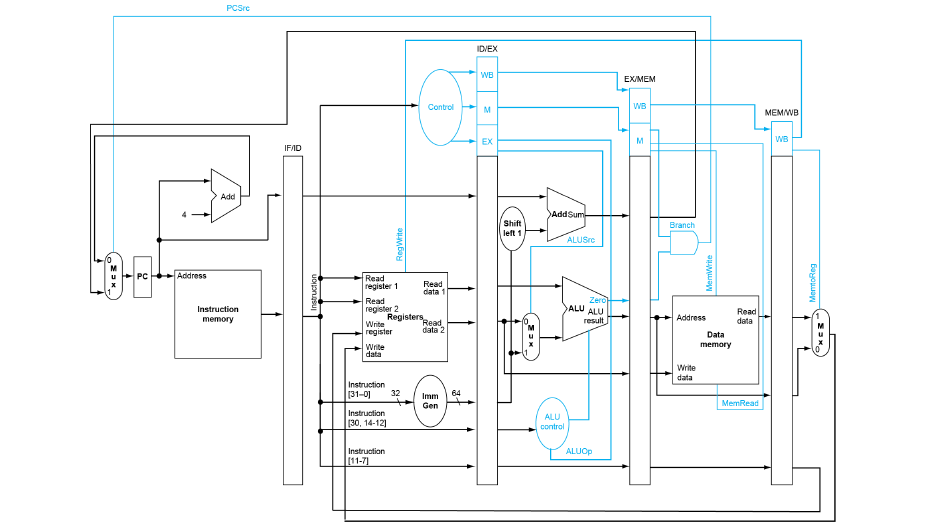
\includegraphics[width=18cm]{./images/structure}
	\caption{General structure}
	\label{fig2.1}
\end{figure}
As requested by the specifications, Instruction and Data memory are not included in the main architecture, however they are implemented it in the testbench.\\
Here we have tried to implement most of the single blocks in a Structural way. \\
Our approach was to describe, where possible, all blocks in a structural manner, so that some parts gain in performance (for instance the branch target adder is built using a CSEA structure instead of using the "+" operand inside a process).
Only Register File, ALU and all Filp-flops are implemented as Behavioral.\\
\\
On Figure \ref{fig2.2} it is showed how we have organized the VHDL files.
\begin{figure}[h!]
	\centering
	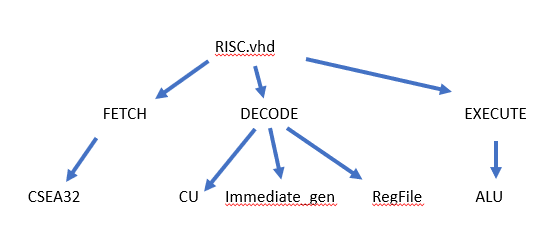
\includegraphics[width=15cm]{./images/VHDL_structure}
	\caption{General VHDL structure}
	\label{fig2.2}
\end{figure}
Now more details on the singular block implementation.
\section{Fetch}
\begin{figure}[h!]
	\centering
	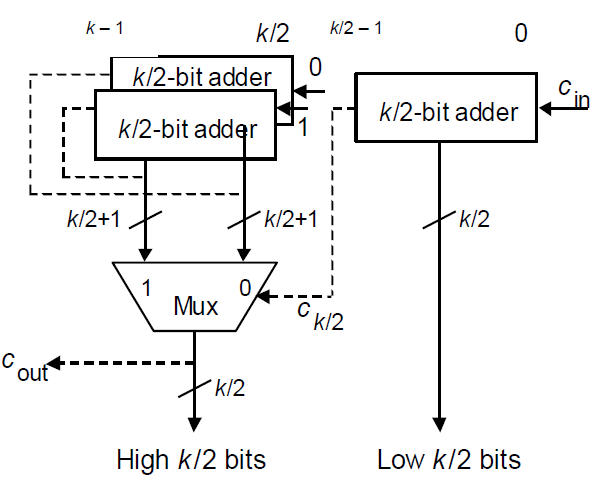
\includegraphics[width=10cm]{./images/CSEA}
	\caption{CSEA structure}
	\label{fig2.3}
\end{figure}
To update the PC we have implemented a Carry Select Adder. \\
Each singular block is composed of a 8 bit Ripple carry adder, in this way the carry propagation delay is reduced.
\section{Decode}
The register file is described in a behavioral manner and it is composed of 32 registers with 32 bit each.\\
When the instruction requires to write data, it will be available only at the next clock cycle in the register. On the other hand, a read operation from a register, is immediately available at the corresponding output.
Ports ReadRegister1 and ReadRegister2 are used to select (using the address at their inputs) a register for the read operation; same for the WriteRegister port that is used for write operations.\\
A write enable signal is used to tell when the RF has to write in the register location.
The register file has the following ports:
\begin{itemize}
	\item Register read1;
	\item Register read2;
	\item WriteRegister;
	\item WriteData;
	\item Read Data1;
	\item Read Data1;
	\item RegWrite;
	\item Reset;
	\item Clock;		
\end{itemize}

The Immediate\_generate block simply reads the instruction and generates a Immediate value (using bit extension).
\begin{figure}[h!]
	\centering
	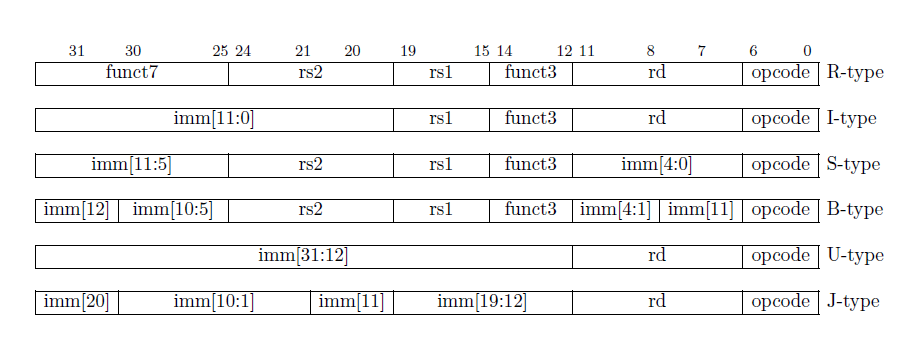
\includegraphics[width=10cm]{./images/immediate_gen}
	\caption{Instruction organization}
	\label{fig2.4}
\end{figure} 
So based on which instruction we are decoding, it organizes a 32 bits Immediate value.
Here we have placed the Control Unit, see next chapter for further details.
\section{Execute}
The adder that creates the new program counter is again implemented with a 32 bits CSEA.
Then we have the ALU that receives two inputs values and the Opcode specifies which instruction should be implemented.\\

In the second version of the processor (that implements the absolute value), we decided to to make the ALU perform the operation, given the proper instruction (that we called ABSV).
More details about the instruction ABSV are described in the Control Unit section of this report.\\

\section{Memory}
This module is described in the RISC top entity. It contains only the AND port that generates the selection signal for the multiplexer on the fetch phase.
\section{Write back}
This module is implemented in the RISC top entity. It contains a four inputs multiplexer and selects between:
\begin{itemize}
	\item Data memory read;
	\item Alu result;
	\item PC + 4 taken from fetch unit;
	\item PC where we need to jump;
\end{itemize}
The last two inputs are considered for the instruction AUIPC and JAL.
The JAL stores the address of the instruction following the jump (pc+4) into register rd.\\
So we take the updated PC in the fetch phase and we bring it in the Write Back phase.\\
AUIPC forms a 32-bit offset from the 20-bit U-immediate and adds this offset to the address of the AUIPC instruction.\\
Then places the result in register rd. 
We take the result in the Execute phase, where with the CSEA we create the branch PC.
\chapter{Control Unit}
The Control Unit is the component that directs the operations of the processor. \\
There are different possibilities for its implementation and we choose the hardwired one: \\
the control hardware it is a finite state machine that switches from a state to another at every clock cycle, generating a sequence of individual bits represent various control signals (i.e. the control word). \\
\\
\begin{figure}[h!]
	\centering
	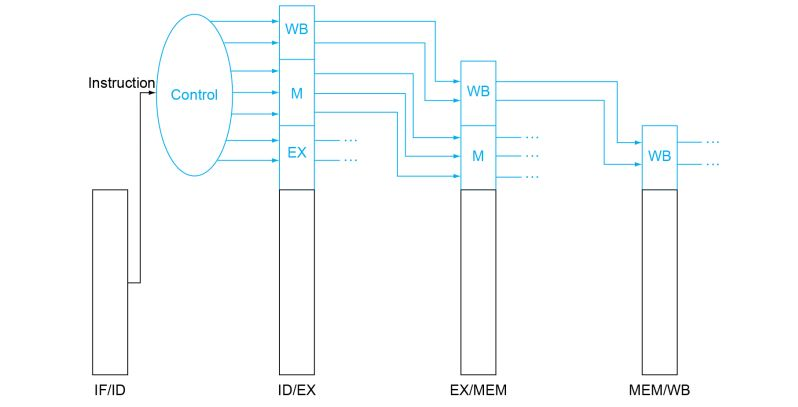
\includegraphics[width=12cm]{./images/structure_CU}
	\caption{General CU structure}
	\label{fig3.1}
\end{figure}

\section{Control Word Generation}
The component receives as input the instruction and based on the instruction's Opcode, it decides which CW it has to send to the output. \\
This selection is based on the bits in position 2, 4, 5, 6. \\
\\
This because we have found that these are the bits which, once concatenated together, identify each instruction uniquely.\\
These bits are used to access to the matrix which generates the corrispondent CW.\\
\begin{figure}[h!]
	\centering
	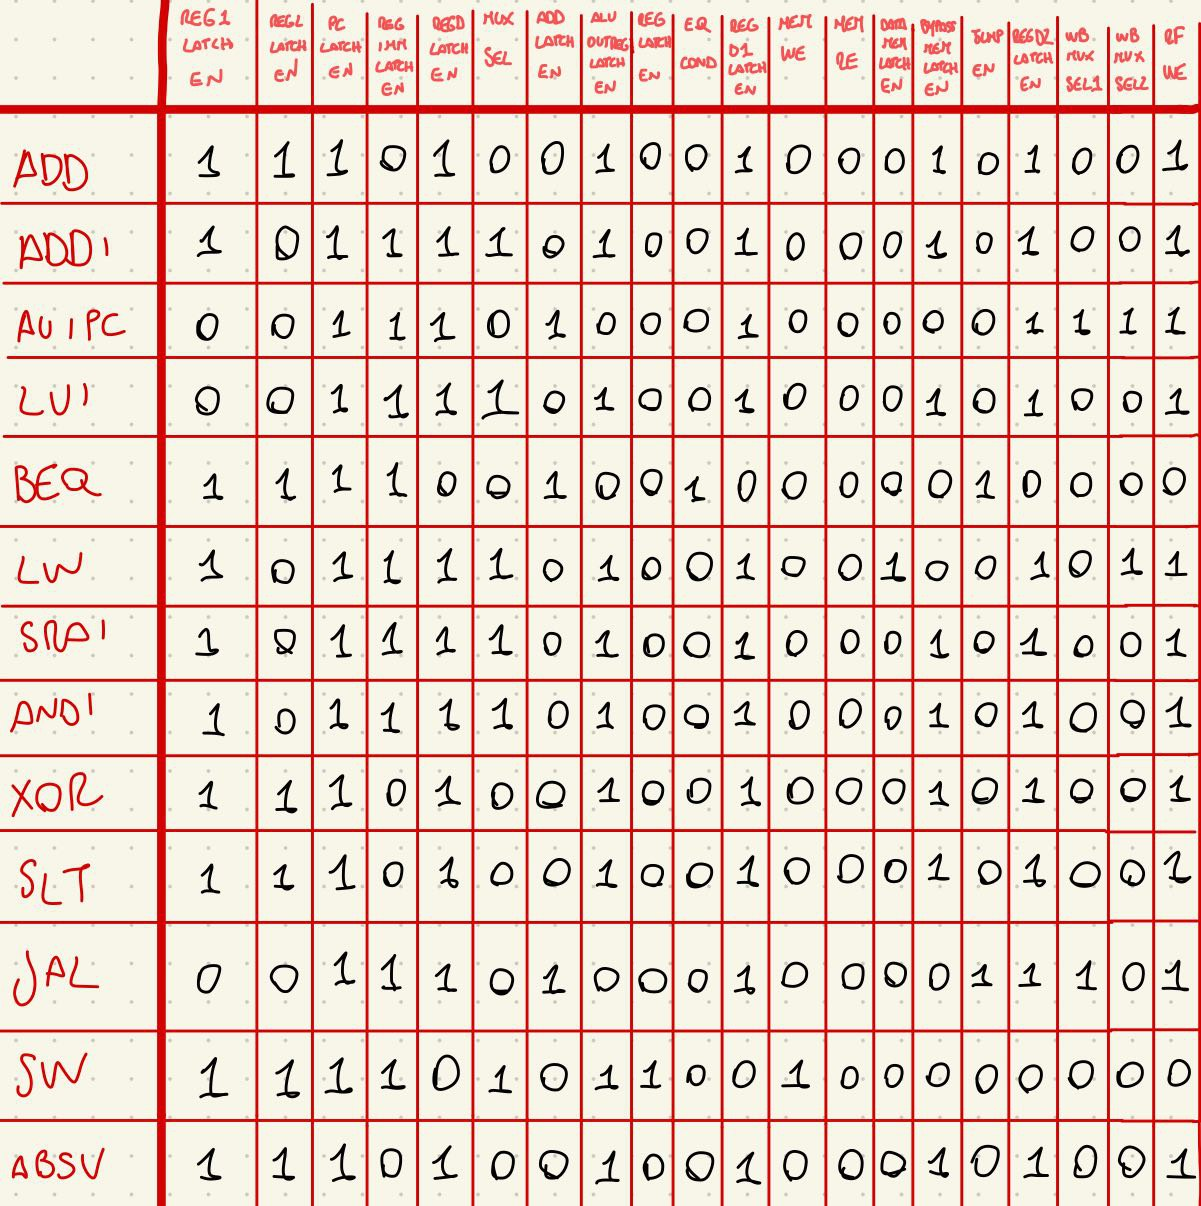
\includegraphics[width=16cm]{./images/control_signals}
	\caption{Control signal of each instruction}
	\label{fig3.3}
\end{figure}
Each instruction has its own control signals, but they are the same for instructions belonging to the same class (exept for some that belong to a class, but they have different control signals):\\
\\
\begin{itemize}
	\item I-type (ADDI, SRAI, ANDI);
	\item LW (I-type);
	\item R-type (ADD, XOR, SLT);
	\item B-type (BEQ);
	\item J-type (JAL);
	\item S-type (SW);
	\item AUIPC (U-type);
	\item LUI (U-type);		
\end{itemize}
\section{ALU Opcode generation}
The second process present in the CU is the one dedicated to the generation of the code destinated to the ALU, in order to determine its behavior.
Its sensitivity list comprehend the instruction's OPCODE and the instruction's FUNCT and it follows the following scheme:\\
\\
\begin{itemize}
	\item I-type -$>$ OPCODE = "0010011" :
		\begin{itemize}
			\item ADDI -$>$ FUNCT = "000";
			\item SRAI -$>$ FUNCT = "101";
			\item ANDI -$>$ FUNCT = "111";
		\end{itemize}
	\item LW (I-type) -$>$ OPCODE = "0000011";
	\item R-type -> OPCODE = "0110011":
		\begin{itemize}
			\item ADD -$>$ FUNCT = "000";
			\item XOR -$>$ FUNCT = "100";
			\item SLT -$>$ FUNCT = "010";
		\end{itemize}
	\item B-type (BEQ) -$>$ OPCODE = "1100011";
	\item J-type (JAL) -$>$ OPCODE = "1101111";
	\item S-type (SW) -$>$ OPCODE = "0100011";
	\item AUIPC (U-type) -$>$ OPCODE = "0010111";
	\item LUI (U-type) -$>$ OPCODE = "0110111";		
\end{itemize}
\chapter{Testbench}
\begin{figure}[h!]
	\centering
	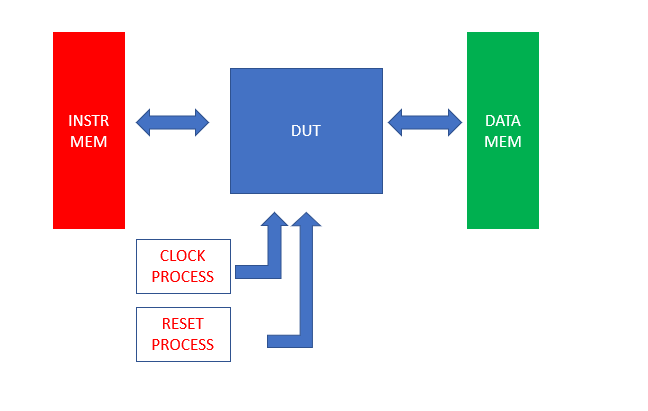
\includegraphics[width=10cm]{./images/Testbench}
	\caption{Testbench organizatiopn}
	\label{fig4.1}
\end{figure} 
The Clock process generate the clock signal for the entire processor.\\
We have decided to adopt a 20ns as a period for the testbench.\\
So our processor is tested at 50MHz. \\
Our goal was to verify that the processor works correctly, withouth considering the performance. \\
For this reason we have used a low frequency.\\
The reset process initialize all the component. This signal is active for 15ns then it is disabled.\\
For what concern the Instruction and Data memory we have implemented both like array of 32 bits.\\
This because both memory are not so big, we have decided to implement them without resorting to a specific structure.\\
\begin{figure}[h!]
	\centering
	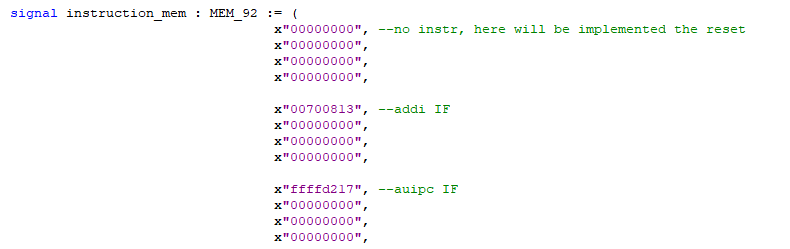
\includegraphics[width=18cm]{./images/Imem}
	\caption{Memory example}
	\label{fig4.2}
\end{figure} 
So for the Instruction memory we have taken the program to test the architecture(Given in the specification)\\
and we have written all the instruction manually. All of them are interleaved by 3 empty instruction, to respect the\\
program counter update(PC+4).
The results are written in the Register file or in the Data memory, depending on which instruction is executed.


\chapter{Synthesis AND Timing}
We have synthetized the architecture and we have created the report for the area and the timing.\\
\section{Area analysis}
Firstly, after the synthesis, we have retrieved the area occupied by our processor.
\begin{figure}[h!]
	\centering
	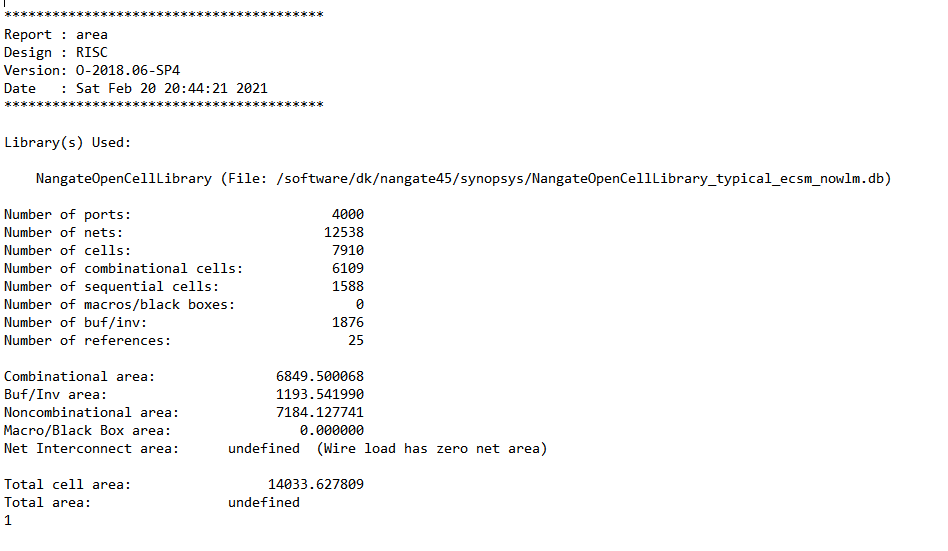
\includegraphics[width=20cm]{./images/RISC_area}
	\caption{Area report}
	\label{fig5.1}
\end{figure} 
\section{Timing analysis}
We have run the synthesis with a clock of 0s. So looking the slack,\\
we can retrieve the maximal clock frequency that our architecture can reach.
Then we have applied that contraint and we have run again the synthesis.\\
Finally we have implemented the routing phase. The result on Figure \ref{fig5.6}.
\begin{figure}[h!]
	\centering
	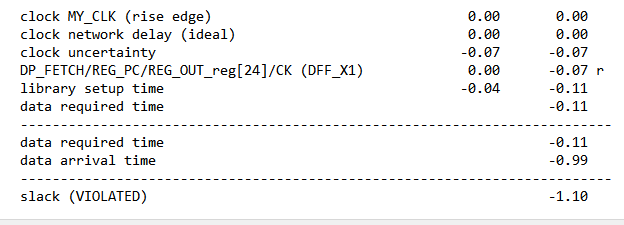
\includegraphics[width=18cm]{./images/RISC_tim0}
	\caption{Timing clock equal to 0}
	\label{fig5.2}
\end{figure}
\begin{figure}[h!]
	\centering
	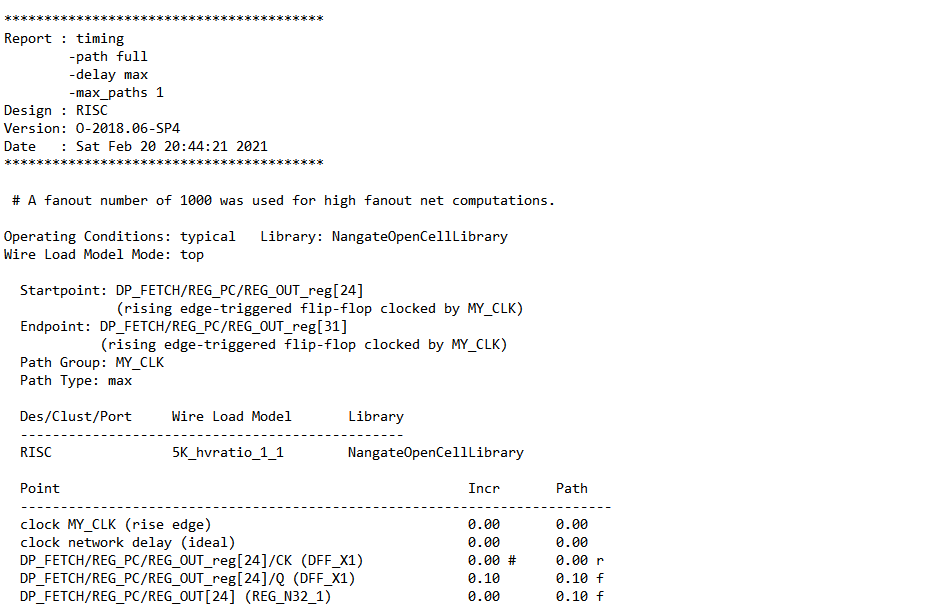
\includegraphics[width=20cm]{./images/RISC_tim1}
	\caption{Timing1}
	\label{fig5.3}
\end{figure}
\begin{figure}[h!]
	\centering
	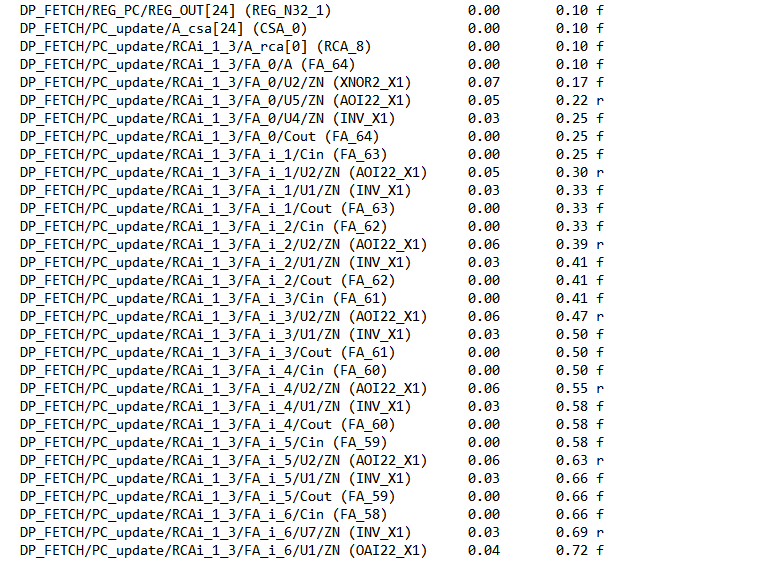
\includegraphics[width=20cm]{./images/RISC_tim2}
	\caption{Timing2}
	\label{fig5.4}
\end{figure}
\begin{figure}[h!]
	\centering
	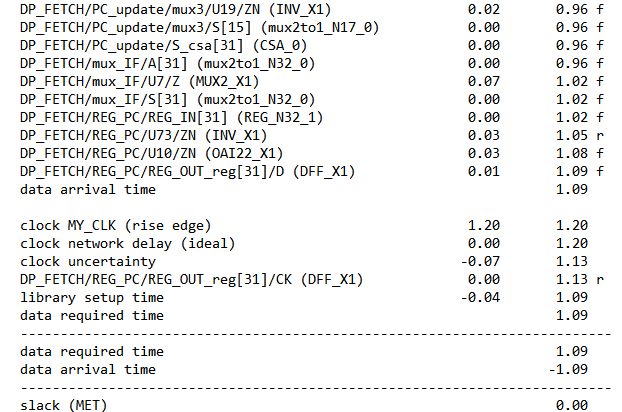
\includegraphics[width=18cm]{./images/RISC_tim3}
	\caption{Timing3}
	\label{fig5.5}
\end{figure}
\begin{figure}[h!]
	\centering
	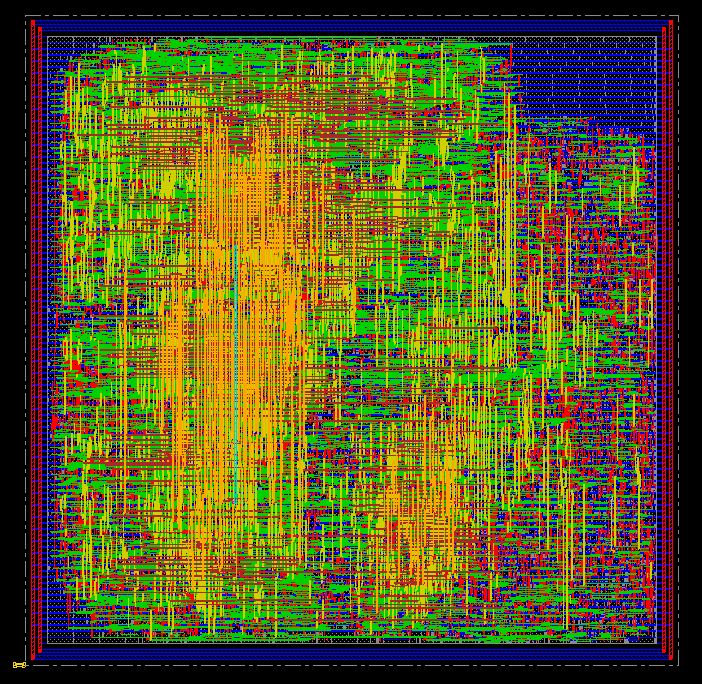
\includegraphics[width=18cm]{./images/original_route}
	\caption{Routing}
	\label{fig5.6}
\end{figure}
%%
%% NOW READ THE FILE master.tex  
\end{document}

